\section*{Exercício 2: Sistema de Classificação de Notas}

\begin{enumerate}
    \item \textbf{Quais testes foram criados?}
    
    Foram concebidos e executados 7 testes unitários automatizados com recurso ao \textit{Pytest} no módulo \texttt{test\_notas.py}, cobrindo todos os cenários obrigatórios e os casos de exceção:
    \begin{itemize}
        \item \texttt{test\_nota\_quatro\_reprovado()}: valida se a nota $4$ retorna a classificação ``Reprovado''.
        \item \texttt{test\_nota\_cinco\_recuperacao()}: valida o limite inferior da faixa de recuperação com a nota $5$.
        \item \texttt{test\_nota\_seis\_nove\_recuperacao()}: valida o limite superior da faixa de recuperação através da nota de fronteira $6{,}9$.
        \item \texttt{test\_nota\_sete\_nove\_aprovado()}:\\ valida o limiar de aprovação através da nota $7$.
        \item \texttt{test\_nota\_dez\_aprovado()}: valida a pontuação máxima da escala com a nota $10$.
        \item \texttt{test\_nota\_negativa\_invalida()}: valida o lançamento de exceção para valores estritamente negativos (ex.: $-15$).
        \item \texttt{test\_nota\_maior\_que\_dez\_invalida()}: \\ valida o lançamento de exceção para valores que excedem a escala (ex.: $15$).
    \end{itemize}

    \begin{figure}[htbp]
        \centering
        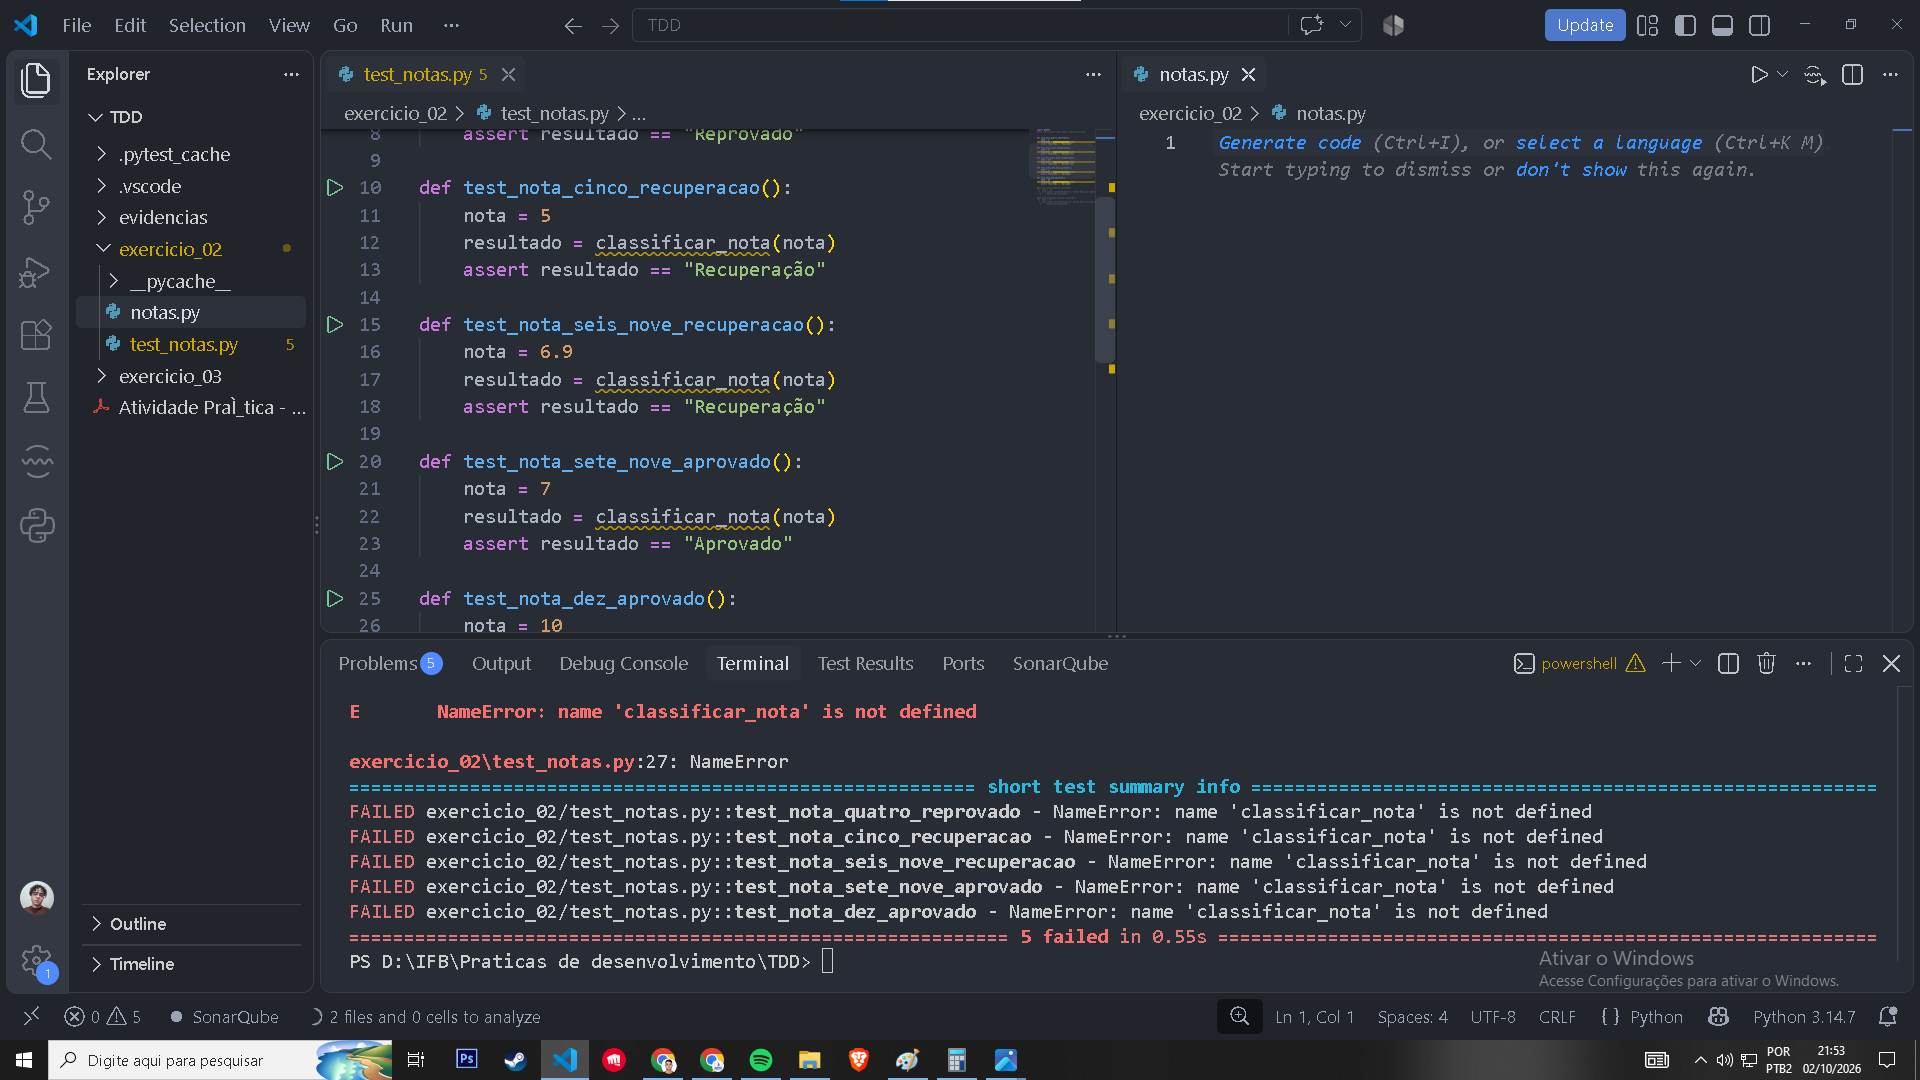
\includegraphics[width=0.92\textwidth]{ex02_red.png}
        \caption{Evidência da fase RED: falha inicial no Pytest (\textit{NameError}) antes da definição da função no módulo.}
        \label{fig:ex02_red}
    \end{figure}

    \item \textbf{Qual caso de teste apresentou maior dificuldade?}
    
    A maior exigência técnica residiu na validação dos casos de fronteira (\textit{boundary value analysis}), com particular destaque para o limite superior da faixa de recuperação na nota $6{,}9$ em transição direta para a nota $7$ (aprovação). Foi necessário garantir que a lógica condicional em \texttt{notas.py} operasse com operadores relacionais adequados (\texttt{nota < 7}), evitando desvios com números decimais. Paralelamente, a estruturação dos testes para verificar o disparo e a captura correta de exceções demandou o uso rigoroso do gestor de contexto \texttt{pytest.raises}.

    \begin{figure}[htbp]
        \centering
        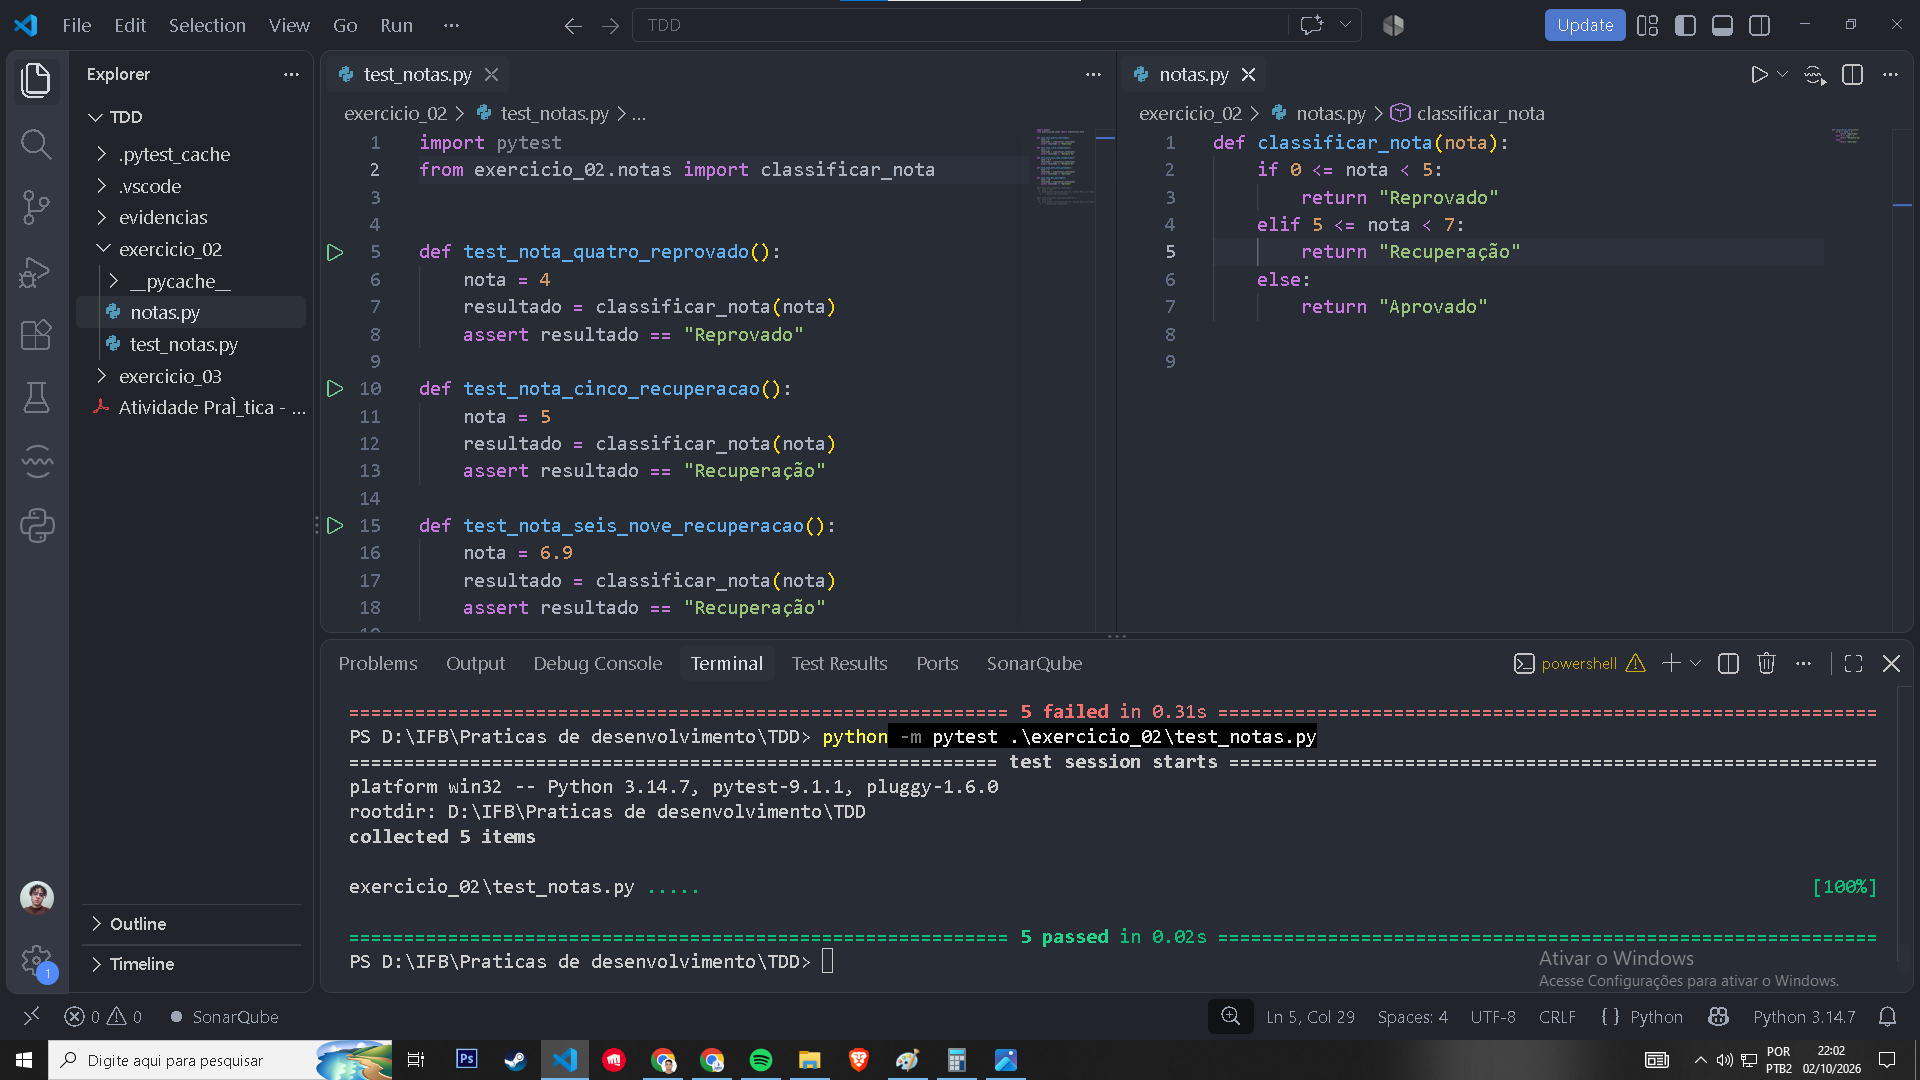
\includegraphics[width=0.92\textwidth]{ex02_green.png}
        \caption{Evidência da fase GREEN: bateria com os 5 casos de teste de classificação obrigatórios aprovados.}
        \label{fig:ex02_green}
    \end{figure}

    \item \textbf{Como você tratou notas inválidas?}
    
    O tratamento de entradas inválidas (valores estritamente inferiores a zero ou superiores a dez) foi feito via lançamento explícito da exceção \texttt{ValueError} seguida da descrição \texttt{"Nota inválida"}. Seguindo o fluxo TDD, foram criados previamente os testes com \texttt{with pytest.raises(ValueError, match="Nota inválida")}, observada a sua falha e, a seguir, criada a cláusula de guarda no módulo \texttt{notas.py}. A execução confirmou a passagem integral da suíte de testes completa.

    \begin{figure}[htbp]
        \centering
        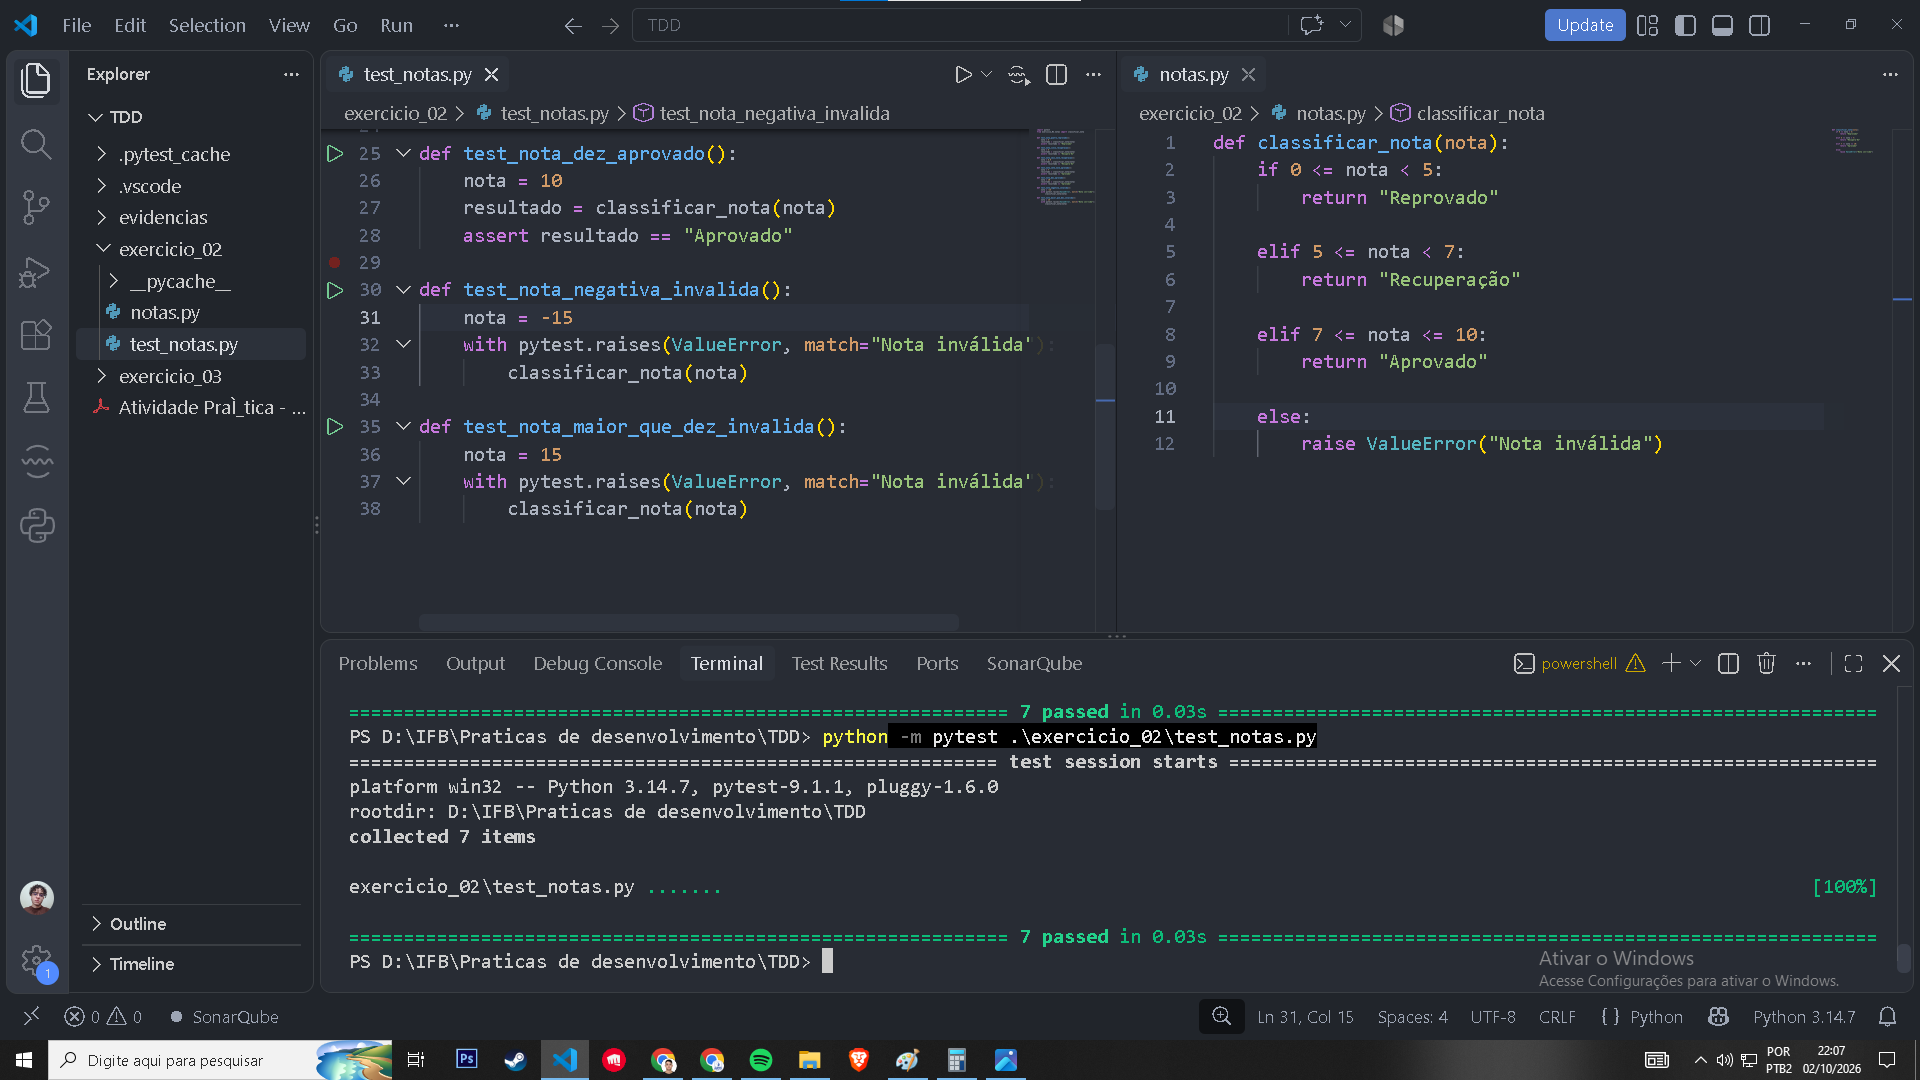
\includegraphics[width=0.92\textwidth]{ex02_refactor.png}
        \caption{Evidência da fase REFACTOR: suíte completa com os 7 testes executados com sucesso no Pytest.}
        \label{fig:ex02_refactor}
    \end{figure}
\end{enumerate}